\section{Simulations}
\label{sec:al:simulations}

We utilize a simulation study in order to determine the method that is 
best-suited for usage with the VS in Chapter~\ref{ch:usage}'s equity 
application. To recap, these are key features of the visualization system that 
should be (and are) captured in the simulations:

\tablespacing
\begin{itemize}
	\item \textbf{Initialization (Section 
	~\ref{sec:visualizer:al:initialization}):} 
	Initializing the active learner begins with a random selection of $k$ data 
	that is presented to the oracle for classification. Each simulation is 
	initialized with 10 randomly selected data points.
	\item \textbf{Pool-based sampling (Section ~\ref{sec:al:litreview}):} After 
	initialization, $k$ unlabeled samples are randomly selected from $X$, and 
	the active learner picks one to query. Each simulation iteration (of the AL 
	algorithm) is presented 15 unlabeled points to query from.
	\item \textbf{Random forest 
	(Section~\ref{sec:visualizer:plotgeneration:tree}):} The VS's overall 
	classification model (for use when initialization and querying are 
	complete) is a random forest. Each active learning method in the 
	simulations optimize for the 
	final random forest classification model by utilizing random forests in 
	their selection process (excluding QBC due to the nature of the 
	algorithm). Instead, the QBC simulations have been run with a committee of 
	classification models that includes random forest (See 
	Section~\ref{sec:al:simulation:methods} for the full list). Furthermore, 
	the QBC simulations have been run with both (1) majority vote and (2) 
	random forest as the overarching classification, as well as (1) with 
	pruning and (2) without pruning.
	\item \textbf{Bivariate classification:} The classification of user 
	interests have two possible labels/levels: ``interesting'' and ``not 
	interesting''. The simulations also use data with two levels of 
	classification (Section~\ref{sec:al:simulation:data}).
\end{itemize}
\bodyspacing

\noindent Finally, it should be noted that each active learning algorithm is 
given a budget of 50 queries (50 progressive iterations of a single trial).

\subsection{Data}
\label{sec:al:simulation:data}
The data is taken from the MNIST database of handwritten digits 
(\url{http://yann.lecun.com/exdb/mnist/}). The digits $(0,1,...,9)$ have 
already been classified and may be visualized in the form of a $28\times 28$ 
pixel array; the darkness of each pixel is represented by a value from 0 
(light) to around 300 (dark). Each image has been transformed into a single 
784-length vector by ``unfurling'' each row and adding it to the last column of 
the row above it. For ease of use and computation efficiency, the data has been 
further compressed to a 196-length vector ($14\times 14$ pixel image). In order 
to maintain the condition of bivariate classification, two out of ten digits 
were selected. The digits 7 and 9 were selected as they are rather similar, 
making it more difficult for an active learning algorithm to correctly parse 
the data with few queries (As opposed to 1 and 0, which are very different on 
the visual plane). The MNIST training set contains 60,000 total data points 
while the testing set contains 10,000 total data points. This was far too many, 
so the simulator selects 250 random samples (125 of each digit) from the 
training set to make up the final data. The final dataset may be visualized in 
Figure~\ref{fig:al:simulations:data}. The functions for working with the MNIST 
data were adapted from file \texttt{gist:39760}~\cite{oconnor2008} and may be 
found in Appendix~\ref{sec:appendicies:al:simulations:data}.

\begin{figure}[htb]
	\begin{center}
		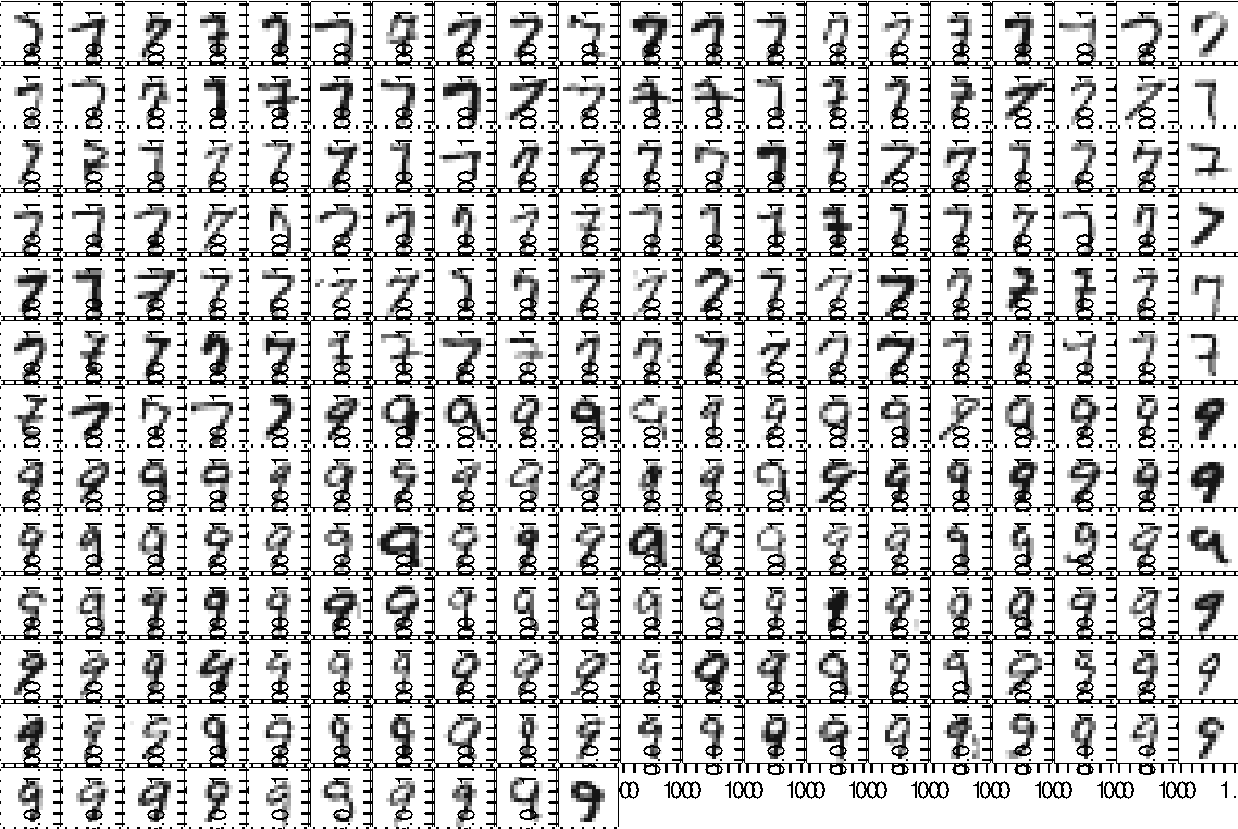
\includegraphics[width=1\linewidth]{ch-al/figures/data.pdf}
		\caption[MNIST data used in the simulations.]{MNIST data used in the 
		simulations. The digits 7 and 9 are relatively similar visually, making 
		the simulations more realistic as it is harder for the classificaiton 
		models to tell the difference.}
		\label{fig:al:simulations:data}
	\end{center}
\end{figure}

\subsection{Evaluation}
\label{sec:al:simulation:evaluation}
The performance of a learner at any given point in time (at any iteration 
\textit{i} of simulation number $k \in [1,25]$) is encapsulated in its error 
ratio $\epsilon$. That is, given the current labeled set, the \textbf{main 
classifier (Random Forest model)} is trained, and the entire dataset is 
predicted given the current classifier. The predictions are stored in an 
$n$-length vector $p$. 
We know the true labels ahead of time (thanks to the MNIST dataset), and they 
are stored in an $n$-length vector $y'$. The predictions are compared against 
the true labels and the error ratio of iteration $i$ is given by
$$\epsilon_i = \frac{1}{250} \bigg( \sum\limits_{z=1}^{250} 
\textbf{1}_{p_z \neq y'_z} \bigg)$$

\noindent where $\textbf{1}_{p_z \neq y'_z}$ is an indicator variable that is 1 
when $p_z \neq y'_z$ and 0 otherwise. These 50 error ratios then form one 
vector $\epsilon_s$, the result of trial 
$s$. To select the best active learning algorithm \textit{on average}, each 
algorithm's error ratios are averaged over 25 total trials. This helps offset 
the randomness of the initialization and pooling scheme. Then the final error 
ratio of an algorithm is given by
$$\epsilon = \frac{1}{25} \bigg( \sum\limits_{i=1}^{25} \epsilon_s \bigg)$$

The final framework for computing $\epsilon_s$, a single trial's vector of 
error ratios, is summarized as follows (This procedure is encapsulated by the 
simulation engine code in 
Appendix~\ref{sec:appendicies:al:simulations:simengine}):

\tablespacing
\begin{algorithm}[H]
	\caption{Computing $\epsilon_s$, a single trial's vector of error 
	ratios}\label{alg:al:simulation:evaluation}
	\begin{algorithmic}[1]
		\Procedure{}{$X$ is a $n\times d$ matrix of $d$ observations of all $n$ 
			variables, $y$ is an $n$-length vector of labels for each variable 
			in $X$ ($y_i$=N/A when $X_{i,}$ has no label). $y'$ is an 
			$n$-length vector of \textbf{true} labels for each variable in $X$. 
			$iter$ is the maximum number of queries allowed per trial}
		\State \textbf{loop from} $i=1$ \textbf{to} $iter$:
		\State \indent $idx \gets $ active\_learning\_method$(X,y,...)$
		\State \indent \textsc{Query} $X_{idx,}$
		\State \indent $tout \gets 
		\text{train}(X^{labeled},y^{labeled},\text{randomforest})$
		\State \indent $p \gets \text{predict}(tout,X)$
		\State \indent $res_i\gets \frac{\text{length}(\text{which}(p \neq y'))}
		{\text{length}(y')}$
		\State \textbf{return} $res$
		\EndProcedure
	\end{algorithmic}
\end{algorithm}
\bodyspacing

\subsection{Summary of methods}
\label{sec:al:simulation:methods}

What follows is a summary of the active learning methods used in the simulation 
with details such tuning parameter values.

\tablespacing
\begin{longtable}{p{0.15\linewidth} p{0.21\linewidth} p{0.18\linewidth} 
p{0.4\linewidth}}
	
	% First page heading
	\caption[Summary of simulation active learning methods.]{A summary of the  
	active learning methods tested in the simulation. *\textit{Note:} The 
	classification model is the main classification model that is used to fit 
	the error, not the classification model(s) used in the active learning 
	methods (those are parameters). 
	The classification model in the simulator is akin to the main 
	classification model in the VS.} 
	\label{tab:al:simulations}\\
	\toprule
	\textbf{AL method} & \textbf{Simulations} & 
	\textbf{Classification model*} & \textbf{Parameters} \\
	\midrule
	\endfirsthead
	
	% Future page heading
	\caption[]{(continued)}\\
	\toprule
	\textbf{AL method} & \textbf{Simulations} & \textbf{Main classification 
	model} & \textbf{Parameters} \\
	\midrule
	\endhead
	
	% Page footer
	\midrule
	\multicolumn{4}{r}{(Continued on next page)}\\
	\endfoot
	
	% Last page footer
	\bottomrule
	\endlastfoot
	
	Random \newline sampling \newline (CONTROL) & 
	25 trials, 50 iterations (queries allowed) each & 
	Random forest & 
	\textit{Classifier}: None \\
	
	\cmidrule[0.1pt](l{0.5em}r{0.5em}){1-4}	
	
	Uncertainty \newline sampling ~\ref{sec:al:methods:uncertainty} & 
	25 trials, 50 iterations (queries allowed) each & 
	Random forest & 
	\textit{Classifier}: Random forest \\

	\cmidrule[0.1pt](l{0.5em}r{0.5em}){1-4}
	
	Query by \newline committee ~\ref{sec:al:methods:qbc} & 
	25 trials, 50 iterations (queries allowed) each & 
	Random forest &	
	\textit{Committee}: RF, NB, SVM, PLS, \newline 
	\textit{Disagreement}: Vote entropy, \newline 
	\textit{C\_Pruning}: T, $\epsilon$: 0.5 \\ & \\
	
	& & Majority \newline committee \newline vote &	
	\textit{Committee}: RF, NB, SVM, PLS, \newline 
	\textit{Disagreement}: Vote entropy, \newline 
	\textit{C\_Pruning}: T, $\epsilon$: 0.5 \\ & \\
	
	& & Random forest &	
	\textit{Committee}: RF, NB, SVM, PLS, \newline 
	\textit{Disagreement}: Vote entropy, \newline 
	\textit{C\_Pruning}: F, $\epsilon$: N/A \\ & \\
	
	& & Majority \newline committee \newline vote &	
	\textit{Committee}: RF, NB, SVM, PLS, \newline 
	\textit{Disagreement}: Vote entropy, \newline 
	\textit{C\_Pruning}: F, $\epsilon$: N/A \\	
	
	\cmidrule[0.1pt](l{0.5em}r{0.5em}){1-4}	
	
	Query by \newline bagging ~\ref{sec:al:methods:bagging} & 
	25 trials, 50 iterations (queries allowed) each & 
	Random forest &
	\textit{Classifier}: Random forest, \newline \textit{Disagreement}: Vote 
	entropy, \newline \textit{num\_class}: 5, \textit{r}: 0.75 \\
		
	\cmidrule[0.1pt](l{0.5em}r{0.5em}){1-4}	
	
	Min-max \newline clustering ~\ref{sec:al:methods:clustering} & 
	25 trials, 50 iterations (queries allowed) each & 
	Random forest & 
	\textit{Classifier}: None, \newline \textit{Distance}: Euclidean \\
	
\end{longtable}
\bodyspacing

A summary of each classification model used in the stating committee for QBC 
implementation is as follows:

\tablespacing
\begin{itemize}
	\item \textbf{Random Forest:} A random forest is a collection of decision 
	trees which are grown from independent draws of the training set. A more 
	detailed description can be found in 
	Section~\ref{sec:visualizer:plotgeneration:tree}.
	\item \textbf{Naive Bayes:}
	\item \textbf{SVM:}
	\item \textbf{Partial Least Squares:}
\end{itemize}
\bodyspacing

The call to each active learning function is controlled by the AL engine code 
in Appendix~\ref{sec:appendicies:al:simulations:alengine}. By implementing the 
active learning call in this way, the main AL functions are hidden from the end 
user so that they cannot call the functions directly, which may lead to 
bypassing checks and/or improperly calling functions.



\subsection{Results}
\label{sec:al:simulation:results}

The full simulator which calls the aforementioned engines, runs the 25 
simulations, and plots the results may be found in 
Appendix~\ref{sec:appendicies:al:simulations:results}.
The results are summarized in the line plot below.

(Discuss how QBC actually spikes up when the pruning occurs, contrary to 
intuition - perhaps there is room for a future extension there. Note that the 
simulations are in no way completely comprehensive/exhaustive, and there is 
further work 
to be done ... For example, trying other classification models within the 
active learning algorithms - who knows, maybe that would've been better! Or 
trying different QBC committees, different tuning parameters i.e. pruning 
factor is 0.75 instead of 0.5, or you prune later/earlier)